\section{PointNet}

\begin{frame}[c]{Introduction to PointNet}
    \large
    \begin{multicols}{2}
        \begin{itemize}
            \item End-to-end learning for unordered point cloud data
            \item Unified framework for previously seperate and specialized tasks
                \begin{itemize}
                    \item Object Classification
                    \item Object Part Segmentation
                    \item Semantic Scene parsing
                \end{itemize}
        \end{itemize}
        \begin{figure}
            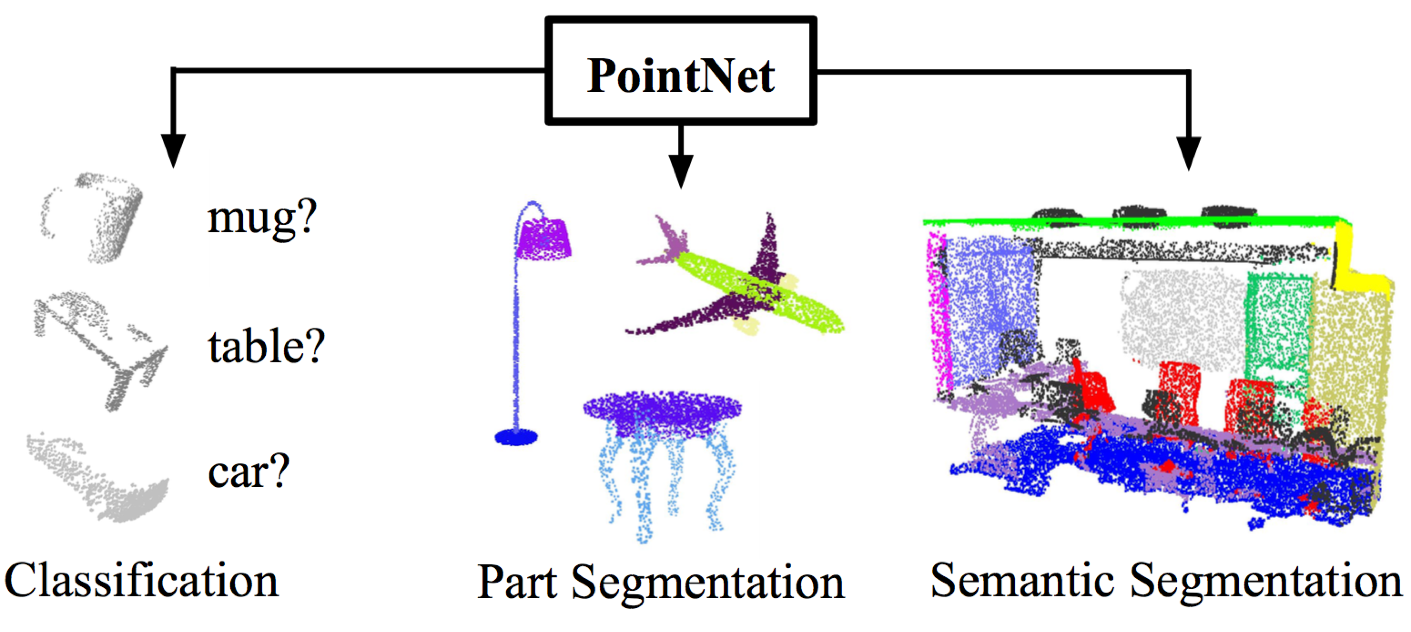
\includegraphics[width=0.5\textwidth]{p12_29}
            \caption{Figure from \cite{qi2017pointnet}.}
        \end{figure}
    \end{multicols}
    \pnote{
        Ergebnis davon: PointNet, einheitliche \\
        architektur für verschiedene Aufgaben
        \par
        Ende-zu-Ende lernen für Punktwolken \\
        Vereinheitlichen von zuvor spezialisierten Aufgaben
    }
\end{frame}


\begin{frame}[c]{Challenges}
    \Large
    \begin{multicols}{2}
        \begin{itemize}[<+->]
            \item Unordered point sets as input
                \begin{itemize}[<1->]
                    \item Model needs to be invariant to $N!$ permutations
                \end{itemize}
            \item Invariance under geometric transformations
                \begin{itemize}[<2->]
                    \item Geometric transformations applied to point cloud data
                        should not alter classification results
                \end{itemize}
        \end{itemize}
        \centering
        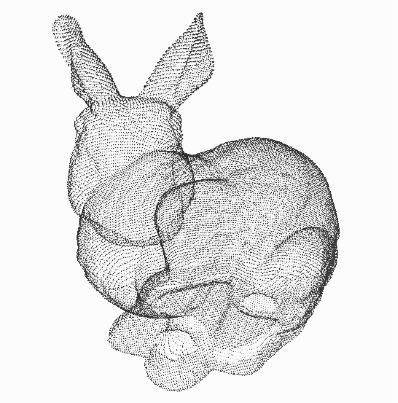
\includegraphics[height=0.35\textheight]{p04_12}
        \includegraphics<2->[height=0.35\textheight]{geometric_transformations}
    \end{multicols}
    \blfootnote{Point cloud figure from CVPR presentation to \cite{qi2017pointnet}.}
    \blfootnote{Geometric transformation figure from \cite{BibEntry2019Oct}.}
    \pnote{
        Herausforderung: Umgang mit Punktwolken. Muss: \\
        - Unsortierte Mengen als eingabe \\
        - Keine Kanonische Höherdimensionale Sortierung \\
        - Invarianz über Geometrische Transformationen
    }
\end{frame}
